\documentclass{bmcart}

%%%%%%%%%%%%%%%%%%%%%%%%%%%%%%%%%%%%%%%%%%%%%%
%%                                          %%
%% CARGA DE PAQUETES DE LATEX               %%
%%                                          %%
%%%%%%%%%%%%%%%%%%%%%%%%%%%%%%%%%%%%%%%%%%%%%%

%%% Load packages
\usepackage{amsthm,amsmath}
\usepackage{graphicx}
%\RequirePackage[numbers]{natbib}
%\RequirePackage{hyperref}
\usepackage[utf8]{inputenc} %unicode support
%\usepackage[applemac]{inputenc} %applemac support if unicode package fails
%\usepackage[latin1]{inputenc} %UNIX support if unicode package fails
\usepackage{hyperref}
\usepackage{float}


\begin{document}

	\begin{frontmatter}
	
		\begin{fmbox}
			\dochead{Research}
			
			%%%%%%%%%%%%%%%%%%%%%%%%%%%%%%%%%%%%%%%%%%%%%%
			%% INTRODUCIR TITULO PROYECTO               %%
			%%%%%%%%%%%%%%%%%%%%%%%%%%%%%%%%%%%%%%%%%%%%%%
			
			\title{Estudio fenotípico del gen HP:0030880 asociado al fenómeno de Raynaud}
			
			%%%%%%%%%%%%%%%%%%%%%%%%%%%%%%%%%%%%%%%%%%%%%%
			%% AUTORES. METER UNA ENTRADA AUTHOR        %%
			%% POR PERSONA                              %%
			%%%%%%%%%%%%%%%%%%%%%%%%%%%%%%%%%%%%%%%%%%%%%%
			
			\author[
			  addressref={aff1},                   % ESTA LINEA SE COPIA IGUAL PARA CADA AUTOR
			  corref={aff1},                       % ESTA LINEA SOLO DEBE TENERLA EL COORDINADOR DEL GRUPO
			  email={jaldanam21@uma.es}   % VUESTRO CORREO ACTIVO
			]{\inits{J.A.M.}\fnm{Jesús} \snm{Aldana}} % inits: INICIALES DE AUTOR, fnm: NOMBRE DE AUTOR, snm: APELLIDOS DE AUTOR
			\author[
			  addressref={aff1},
			  email={juancaruru@uma.es}
			]{\inits{J.C.}\fnm{Juan Carlos} \snm{Ruiz}}
			
			%%%%%%%%%%%%%%%%%%%%%%%%%%%%%%%%%%%%%%%%%%%%%%
			%% AFILIACION. NO TOCAR                     %%
			%%%%%%%%%%%%%%%%%%%%%%%%%%%%%%%%%%%%%%%%%%%%%%
			
			\address[id=aff1]{%                           % unique id
			  \orgdiv{ETSI Informática},             % department, if any
			  \orgname{Universidad de Málaga},          % university, etc
			  \city{Málaga},                              % city
			  \cny{España}                                    % country
		}
		
		\end{fmbox}% comment this for two column layout
		
		\begin{abstractbox}
		
			\begin{abstract} % abstract
			
			%%%%%%%%%%%%%%%%%%%%%%%%%%%%%%%%%%%%%%%%%%%%%%%
			%% RESUMEN BREVE DE NO MAS DE 100 PALABRAS   %%
			%%%%%%%%%%%%%%%%%%%%%%%%%%%%%%%%%%%%%%%%%%%%%%%	
			Esta memoria de investigación se realizó siguiendo la estructura convencional de una revista científica, con el objetivo de divulgar una enfermedad rara que afecta a numerosas personas en nuestro país. Hicimos un estudio acerca de aquellos genes a los que afecta y el fenotipo que producen. Toda la información investigada se organizó en forma de grafo y redes biológicas para su posterior análisis.
						
			This research report was carried out following the conventional structure of a scientific journal, with the aim of disseminating a rare disease that affects many people in our country. We did a study about the genes it affects and the phenotype they produce. All the information investigated was organized in the form of a graph and biological networks for further analysis.
			
			\end{abstract}
			
			%%%%%%%%%%%%%%%%%%%%%%%%%%%%%%%%%%%%%%%%%%%%%%
			%% PALABRAS CLAVE DEL PROYECTO              %%
			%%%%%%%%%%%%%%%%%%%%%%%%%%%%%%%%%%%%%%%%%%%%%%
			
			\begin{keyword}
			\kwd{Raynaud}
			\kwd{gene}
			\kwd{phenotype}
			\kwd{ontology}
			\end{keyword}
		
		
		\end{abstractbox}
	
	\end{frontmatter}
	
	\section{Introducción}

En este proyecto de investigación usaremos ontologías, en concreto GO, para poder conocer las relaciones que tienen los genes a estudiar con el resto. Podemos definir una ontología como una manera formal de representar el conocimiento colectivo sobre un área en la que sus conceptos se describen por su significado y su relación con el resto de componentes[citas], en nuestro caso se trataría de fenotipos y genes. 

Así el proyecto investigará el fenómeno de Raynaud a través de diferentes bases de datos y ontologías para conocer que sistemas y rutas biológicas se ven afectados por esta patología y como se relaciona con el resto de fenotipos conocidos.

\subsection{Fenómeno Raynaud}


	\section{Materiales y métodos}

	\section{Resultados}

\begin{spacing}{1}
Tras la obtención de la red de genes al realizar el mapeo con STRINGdb hemos obtenido un grafo como el que podemos observar en la figura \ref{fig:graph1}. En este grafo podemos observar todos los genes que pertenecen a la red asociada al fénomeno de Raynaud. Esto se ha obtenido a partir de STRINGdb como hemos explicado en el apartado \ref{obtencion_red}.
\end{spacing}

\begin{minipage}{\linewidth}
	\makebox[\linewidth]{
		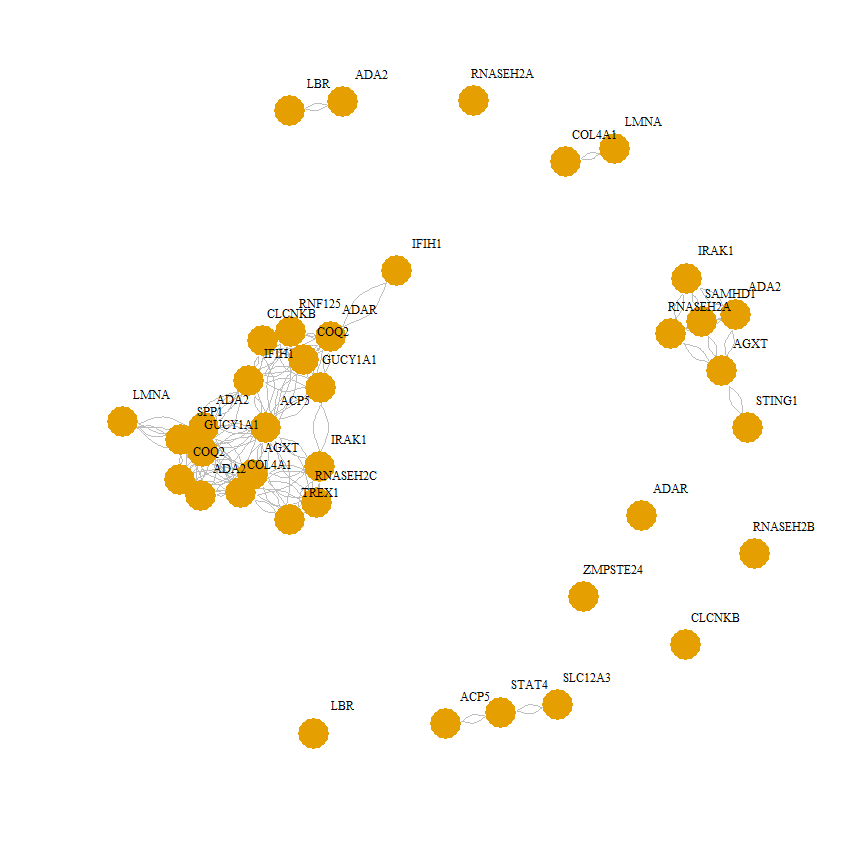
\includegraphics[width=\textwidth]{figures/Raynaud_genes-graph.png}
	}
	\captionof{figure}{Grafo obtenido al realizar el mapeo de genes}
	\label{fig:graph1}
\end{minipage}

\begin{spacing}{1}
	Seguidamente hemos obtenido las comunidades que conforman nuestra red y a las que posteriormente se le harán los estudios de funcionalidad y podremos comprobar que genes conforman el fenotipo más grave de la enfermedad. Se han obtenido 3 gráficas en las que mostramos información acerca de estas comunidades.
	
	En la figura \ref{fig:dendrogram}, la primera obtenida del flujo de trabajo, se observa un dendrograma en la que, diferenciadas por colores, se pueden visualizar las diferentes comunidades obtenidas. Estas se han obtenido a una altura bastante alta (alrededor del 0.9) y nos indica que tenemos 6 comunidades cuyo agrupamiento más grande tiene 11 genes.
\end{spacing}

\begin{minipage}{\linewidth}
	\makebox[\linewidth]{
		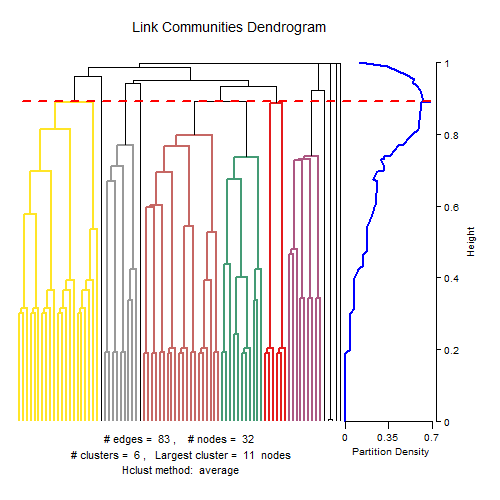
\includegraphics[width=0.7\textwidth]{figures/Raynaud_genes-dendrogram.png}
	}
	\captionof{figure}{Dendrograma de la red mostrando las comunidades}
	\label{fig:dendrogram}
\end{minipage}

\begin{spacing}{1}
La segunda figura que obtenemos del flujo de trabajo sería la número \ref{fig:members}, en esta observamos una matriz de los miembros de cada comunidad. En este caso solo podemos ver los 10 primeros genes de nuestra red y en la matriz se nos muestra las comunidades a las que pertenece cada gen (señalado con un cuadrado en color para cada comunidad a la que pertenece). Además en los márgenes derecho e inferior de la matriz observamos los sumatorios del número de total de comunidades a las que pertenece cada gen y el número de genes que contiene cada comunidad, respectivamente.
\end{spacing}

\begin{minipage}{\linewidth}
	\makebox[\linewidth]{
		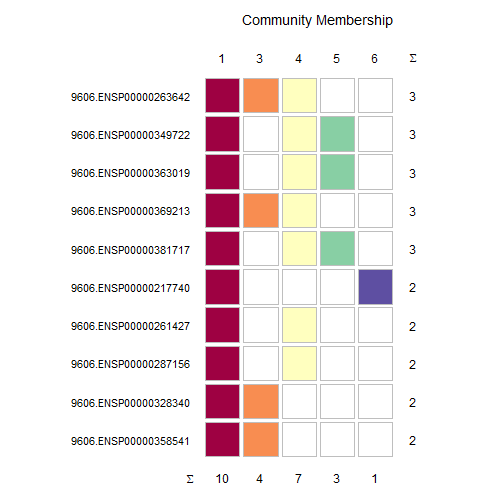
\includegraphics[width=0.7\textwidth]{figures/Raynaud_genes-comunity_members_matrix.png}
	}
	\captionof{figure}{Matriz de los primeros genes para cada comunidad}
	\label{fig:members}
\end{minipage}

\begin{spacing}{1}
	Por último, al obtener las comunidades también hemos mostrado la figura \ref{fig:comunity_graph} en la que se observa un grafo similar al de la figura \ref{fig:graph1}, sin embargo, en este tenemos diferenciadas por colores las diferentes comunidades que hemos obtenido tras realizar el flujo de trabajo.
\end{spacing}

\begin{minipage}{\linewidth}
	\makebox[\linewidth]{
		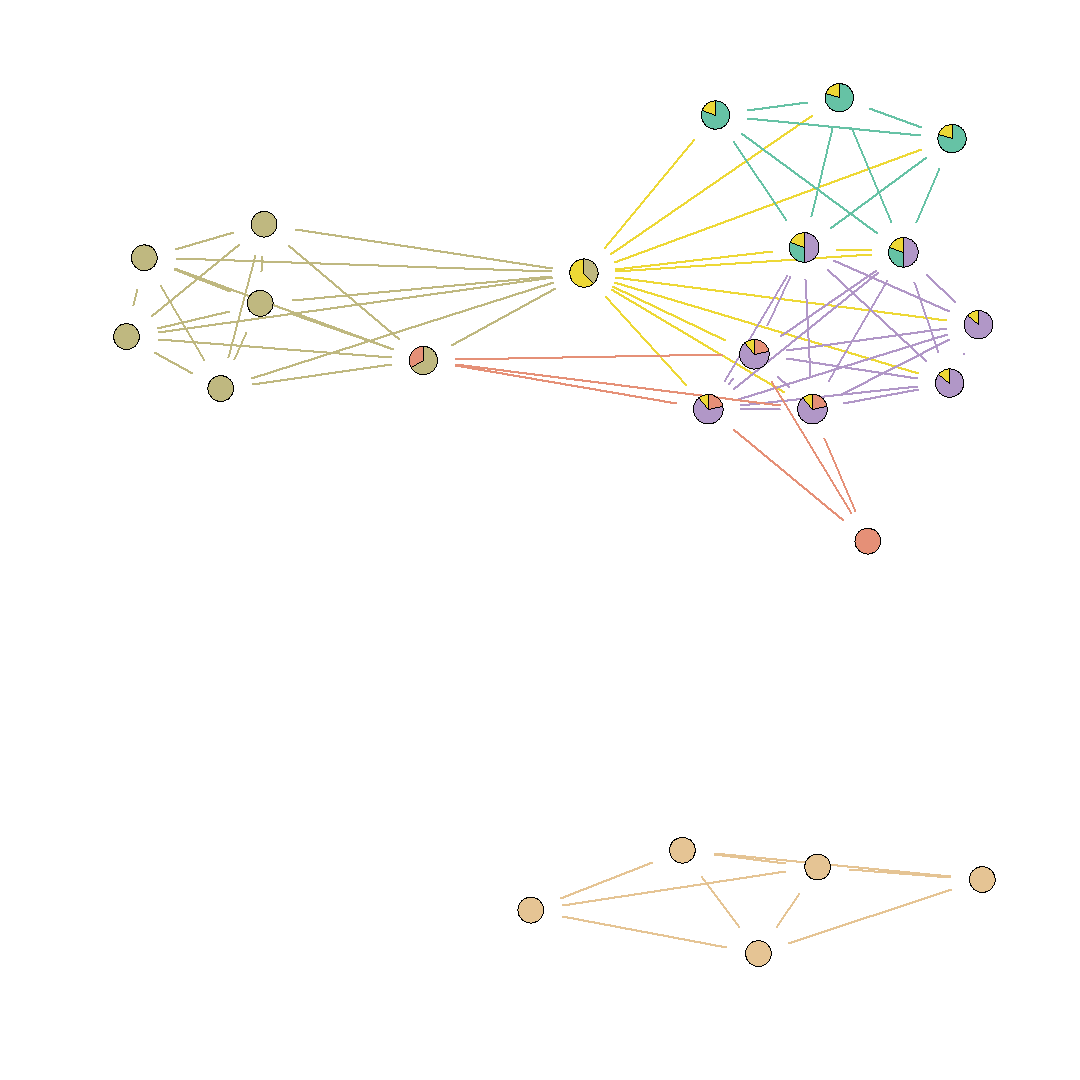
\includegraphics[width=0.7\textwidth]{figures/Raynaud_genes-comunities_graph.png}
	}
	\captionof{figure}{Grafo de los genes divididos por comunidad}
	\label{fig:comunity_graph}
\end{minipage}

\begin{spacing}{1}
Por último, hemos obtenido los CSV de cada una de las comunidades tras aplicarles el enriquecimiento. No todas las comunidades han devuelto una tabla con datos y los datos que sí hemos obtenido podemos observarlos en las tablas \ref{tab:comunity1} y \ref{tab:comunity2}, correspondiendo a las comunidades 1 y 2, respectivamente.

En estas tablas podemos observar las columnas de \textit{Ontología}, que nos indica la ontología de la que se ha obtenido esa referencia; \textit{Término}, que indica el código de la ontología que relaciona a dicho gen; \textit{N genes} y \textit{Genes totales}, que indican el número de genes encontrados y el número de genes que tiene asociado dicho término; en la columna \textit{Genes} vemos los nombres de los genes encontrados; y por último tenemos dos columnas para el \textit{p valor} y el \textit{fdr}, además de una descipción del término de la ontología.
\end{spacing}

\begin{table}[!ht]
	\centering
	\resizebox{\textwidth}{!}{
	\begin{tabular}{|cccccccccc|}
		\hline
		\textbf{Ontología} & \textbf{Categoría} & \textbf{Término} & \textbf{N genes} & \textbf{Genes totales} & \textbf{Taxon Id} & \textbf{genes} & \textbf{p valor} & \textbf{fdr} & \textbf{descripción} \\ \hline
		GO & Process & GO.0032480 & 2 & 43 & 9606 & RNF125,IFIH1 & 5.17e-06 & 0.0011 & negative regulation of type I interferon production \\ 
		GO & Process & GO.0045088 & 2 & 361 & 9606 & RNF125,IFIH1 & 0.00034 & 0.018 & regulation of innate immune response \\ 
		GO & Process & GO.0043900 & 2 & 653 & 9606 & RNF125,IFIH1 & 0.0011 & 0.0347 & regulation of multi-organism process \\ 
		GO & Process & GO.0032446 & 2 & 690 & 9606 & RNF125,IFIH1 & 0.0012 & 0.0347 & protein modification by small protein conjugation \\ \hline
	\end{tabular}
	}
	\vspace{5px}
	\caption{Resultado del enriquecimiento de la comunidad 1}
	\label{tab:comunity1}
\end{table}

\begin{table}[!ht]
	\centering
	\resizebox{\textwidth}{!}{
	\begin{tabular}{|c|ccccccccc|}
		\hline
		\textbf{Ontología} & \textbf{Categoría} & \textbf{Término} & \textbf{N genes} & \textbf{Genes totales} & \textbf{Taxon Id} & \textbf{genes} & \textbf{p valor} & \textbf{fdr} & \textbf{descripción} \\ \hline
		GO & Process & GO.0090305 & 4 & 287 & 9606 & RNASEH2A,SAMHD1,TREX1,RNASEH2B & 2.37e-07 & 4.26e-05 & nucleic acid phosphodiester bond hydrolysis \\ 
		GO & Process & GO.0034655 & 4 & 394 & 9606 & RNASEH2A,SAMHD1,RNASEH2C,RNASEH2B & 8.29e-07 & 7.46e-05 & nucleobase-containing compound catabolic process \\ 
		GO & Process & GO.0090501 & 3 & 137 & 9606 & RNASEH2A,SAMHD1,RNASEH2B & 3.55e-06 & 9.12e-05 & RNA phosphodiester bond hydrolysis \\ 
		GO & Process & GO.0006401 & 3 & 237 & 9606 & RNASEH2A,RNASEH2C,RNASEH2B & 1.79e-05 & 4e-04 & RNA catabolic process \\ 
		GO & Process & GO.0006298 & 2 & 26 & 9606 & RNASEH2A,TREX1 & 1.97e-05 & 4e-04 & mismatch repair \\ 
		GO & Process & GO.0090502 & 2 & 70 & 9606 & RNASEH2A,RNASEH2B & 0.00013 & 0.0024 & RNA phosphodiester bond hydrolysis, endonucleolytic \\ 
		GO & Process & GO.0090304 & 5 & 3941 & 9606 & RNASEH2A,SAMHD1,TREX1,RNASEH2C,RNASEH2B & 0.00033 & 0.0046 & nucleic acid metabolic process \\ 
		GO & Process & GO.0006260 & 2 & 203 & 9606 & RNASEH2A,TREX1 & 0.0011 & 0.01 & DNA replication \\ 
		GO & Process & GO.0016070 & 4 & 3430 & 9606 & RNASEH2A,SAMHD1,RNASEH2C,RNASEH2B & 0.0041 & 0.0318 & RNA metabolic process \\ \hline
	\end{tabular}
	}
	\vspace{5px}
	\caption{Resultado del enriquecimiento de la comunidad 2}
	\label{tab:comunity2}
\end{table}
	\section{Discusión}

Como podemos observar en la figura \ref{fig:dendrogram} de los resultados queremos destacar el cluster número (1/6)

	\section{Conclusiones}

Tal y como pretendíamos en \ref{objetivos} hemos realizado un estudio acerca de los procesos moleculares obtenidos unos resultados muy interesantes de los genes relacionados con el fenómeno de Raynaud como vemos en las tablas de resultados \ref{resultados}. No obstante como ya sabemos el estudio de las enfermedades raras contempla algunas limitaciones debido a la complejidad de las interacciones y los procesos que ocurren en la enfermedad así como la variedad de mutaciones genéticas y combinaciones distintas que dan lugar a las enfermedades raras.

Respecto a nuestro estudio somos conscientes de la falta de datos de seguimiento de pacientes ya que pese a tener multitud de datos a nivel biológico y molecular, entendemos que este tipo de enfermedades se pueden expresar de diferentes maneras según el paciente y puede ser beneficioso buscar terapias a nivel de individuo. \\
\\
Como futuras líneas de investigación creemos que lo más importante sería el desarrollo de nuevas terapias génicas para tratar los síntomas subyacentes al síndrome de Raynaud y un estudio de seguimiento más a largo plazo que nos permita evaluar la efectividad de las terapias y detectar cambios en la condición del paciente y la evolución de la patología. Otra línea para continuar el estudio de este proyecto sería la investigación del catalizador que produce la enfermedad analizando a pacientes de temprana edad para hallar con precisión el origen del fenómeno.
	
	
	%%%%%%%%%%%%%%%%%%%%%%%%%%%%%%%%%%%%%%%%%%%%%%
	%% OTRA INFORMACIÓN                         %%
	%%%%%%%%%%%%%%%%%%%%%%%%%%%%%%%%%%%%%%%%%%%%%%
	
	\begin{backmatter}
	
		\section*{Abreviaciones}%% if any
			\begin{itemize}
				\item \label{GO} \textbf{GO}: Gene Ontology 
				\item \label{HPO} \textbf{HPO}: Human Phenotype Ontology database
				\item  \label{OMIM} \textbf{OMIM}: Online Mendelian Inheritance in Man database
				\item \label{GSEA} \textbf{GSEA}: Gene Sequence Enrinchment Analysis
				\item \label{NASQAR} \textbf{NASQAR}: Nucleic Acid Sequence Analysis Resource
				\item \label{KEGG} \textbf{KEGG}: Kyoto Encyclopedia of Genes and Genomes
			\end{itemize}
		
		\section*{Disponibilidad de datos y materiales}%% if any
			Repositorio de github:
			\href{https://github.com/jesusaldanamartin/Gene_Phenotipycal_Study}{https://github.com/jesusaldanamartin/Gene\_Phenotipycal\_Study}
		
		\section*{Contribución de los autores}
			J.C. : Encargado de la introducción. 
			J.A.M. : Encargado del abstract y parte de la introducción
			%OJO: que sea realista con los registros que hay en vuestros repositorios de github. 
		
		
		%%%%%%%%%%%%%%%%%%%%%%%%%%%%%%%%%%%%%%%%%%%%%%%%%%%%%%%%%%%%%%%%%%%%%%%%%%%%%%%%%%%%%%%%
		%% BIBLIOGRAFIA: no teneis que tocar nada, solo sustituir el archivo bibliography.bib %%
		%% por el que hayais generado vosotros                                                %%
		%%%%%%%%%%%%%%%%%%%%%%%%%%%%%%%%%%%%%%%%%%%%%%%%%%%%%%%%%%%%%%%%%%%%%%%%%%%%%%%%%%%%%%%%
		
		\bibliographystyle{bmc-mathphys} % Style BST file (bmc-mathphys, vancouver, spbasic).
		\bibliography{bibliography.bib}      % Bibliography file (usually '*.bib' )
	
	\end{backmatter}
\end{document}
